% **************************************************
% Document Class Definition
% **************************************************
\documentclass[%
	paper=A4,					% paper size --> A4 is default in Germany
	twoside=true,				% onesite or twoside printing
	openright,					% doublepage cleaning ends up right side
	parskip=full,				% spacing value / method for paragraphs
	chapterprefix=true,			% prefix for chapter marks
	11pt,						% font size
	headings=normal,			% size of headings
	bibliography=totoc,			% include bib in toc
	listof=totoc,				% include listof entries in toc
	titlepage=on,				% own page for each title page
	captions=tableabove,		% display table captions above the float env
	draft=false,				% value for draft version
]{scrreprt}%

% **************************************************
% Debug LaTeX Information
% **************************************************
%\listfiles

% **************************************************
% Information and Commands for Reuse
% **************************************************
\newcommand{\ie}{\textit{i.e.,}\xspace}
\newcommand{\eg}{\textit{e.g.,}\xspace}
\newcommand{\etc}{\textit{etc.}\xspace}
\newcommand{\thesisTitle}{User Interface Test Automation Tools for iOS Applications}
\newcommand{\thesisName}{Alejandro Echeverri Romero}
\newcommand{\thesisSubject}{Proyecto de grado}
\newcommand{\thesisDate}{Diciembre, 2019}
\newcommand{\thesisVersion}{1.0}

\newcommand{\thesisFirstReviewer}{Ph.D. Nicol\'{a}s Cardozo }
\newcommand{\thesisFirstReviewerUniversity}{\protect{Universidad de los Andes, Bogot\'{a}, Colombia}}
\newcommand{\thesisFirstReviewerDepartment}{Departamento de Ingenier\'{i}a de Sistemas y Computaci\'{o}n}

\newcommand{\thesisSecondReviewer}{Ph.D. Gabriele Bavota}
\newcommand{\thesisSecondReviewerUniversity}{\protect{Universit\`{a} della Svizzera italiana (USI), Lugano}}
\newcommand{\thesisSecondReviewerDepartment}{Faculty of Informatics }

\newcommand{\thesisFirstSupervisor}{Ph.D. Mario Linares V\'{a}squez}

\newcommand{\thesisUniversity}{\protect{Universidad de los Andes}}
\newcommand{\thesisUniversityDepartment}{Departamento de Ingenier\'{i}a de Sistemas y Computaci\'{o}n}
\newcommand{\thesisUniversityInstitute}{Facultad de Ingenier\'{i}a}
\newcommand{\thesisUniversityGroup}{The Software Design Lab}
\newcommand{\thesisUniversityCity}{Bogot\'{a}, Colombia}
\newcommand{\thesisUniversityStreetAddress}{Cra 1 \# 18A - 12}
\newcommand{\thesisUniversityPostalCode}{111711}



% **************************************************
% Load and Configure Packages
% **************************************************
\usepackage[T1]{fontenc}
\usepackage[utf8]{inputenc}		% defines file's character encoding
\usepackage[english]{babel} % babel system, adjust the language of the content
\usepackage[					% clean thesis style
	figuresep=colon,%
	sansserif=false,%
	hangfigurecaption=false,%
	hangsection=true,%
	hangsubsection=true,%
	colorize=full,%
	colortheme=bluemagenta,%
	bibsys=bibtex,%
	bibfile=bib-refs,%
	bibstyle=numeric,%
]{cleanthesis}
\usepackage[linesnumbered]{algorithm2e}
\usepackage{adjustbox}
\usepackage{listings,color}
\usepackage{amsfonts}
\usepackage{tcolorbox}
\usepackage{amssymb}
\usepackage{ifthen}
\lstset{
	language=xml,
	tabsize=2,
	%frame=lines,
	frame=shadowbox,
	rulesepcolor=\color{gray},
	xleftmargin=18pt,
	framexleftmargin=15pt,
	keywordstyle=\color{blue},
	commentstyle=\color{OliveGreen},
	stringstyle=\color[rgb]{0,0.43,0.72},
	numbers=left,
	numberstyle=\tiny,
	numbersep=4pt,
	breaklines=true,
	showstringspaces=false,
	basicstyle=\ttfamily\scriptsize,
	columns=fullflexible,
	emph={node,name,price},emphstyle={\color{magenta}}}

\colorlet{punct}{red!60!black}
\definecolor{background}{HTML}{EEEEEE}
\definecolor{delim}{RGB}{20,105,176}
\colorlet{numb}{magenta!60!black}
\lstdefinelanguage{json}{
	basicstyle=\ttfamily\scriptsize,
	numbers=left,
	numberstyle=\scriptsize,
	stepnumber=1,
	numbersep=8pt,
	showstringspaces=false,
	breaklines=true,
	frame=shadowbox,
	literate=
	*{0}{{{\color{numb}0}}}{1}
	{1}{{{\color{numb}1}}}{1}
	{2}{{{\color{numb}2}}}{1}
	{3}{{{\color{numb}3}}}{1}
	{4}{{{\color{numb}4}}}{1}
	{5}{{{\color{numb}5}}}{1}
	{6}{{{\color{numb}6}}}{1}
	{7}{{{\color{numb}7}}}{1}
	{8}{{{\color{numb}8}}}{1}
	{9}{{{\color{numb}9}}}{1}
	{:}{{{\color{punct}{:}}}}{1}
	{,}{{{\color{punct}{,}}}}{1}
	{\{}{{{\color{delim}{\{}}}}{1}
	{\}}{{{\color{delim}{\}}}}}{1}
	{[}{{{\color{delim}{[}}}}{1}
	{]}{{{\color{delim}{]}}}}{1},
}

\lstloadlanguages{xml}
\renewcommand{\lstlistingname}{Code example}% Listing -> Algorithm
\renewcommand{\lstlistlistingname}{List of \lstlistingname s}


\hypersetup{					% setup the hyperref-package options
	pdftitle={\thesisTitle},	% 	- title (PDF meta)
	pdfsubject={\thesisSubject},% 	- subject (PDF meta)
	pdfauthor={\thesisName},	% 	- author (PDF meta)
	plainpages=false,			% 	-
	colorlinks=false,			% 	- colorize links?
	pdfborder={0 0 0},			% 	-
	breaklinks=true,			% 	- allow line break inside links
	bookmarksnumbered=true,		%
	bookmarksopen=true			%
}

\newcommand{\nb}[2]{
	\fbox{\bfseries\sffamily\scriptsize#1}
	{\small$\blacktriangleright$\textit{#2}$\blacktriangleleft$}}
\newcommand\MARIO[1]{\textcolor{red}{\nb{MARIO}{#1}}}
\newcommand\SANTIAGO[1]{\textcolor{orange}{\nb{SANTIAGO}{#1}}}
% **************************************************
% Document CONTENT
% **************************************************
\begin{document}

% --------------------------
% rename document parts
% --------------------------
%\renewcaptionname{ngerman}{\figurename}{Abb.}
%\renewcaptionname{ngerman}{\tablename}{Tab.}
\renewcaptionname{english}{\figurename}{Fig.}
\renewcaptionname{english}{\tablename}{Tab.}

% --------------------------
% Front matter
% --------------------------
\pagenumbering{roman}			% roman page numbing (invisible for empty page style)
\pagestyle{empty}				% no header or footers
% !TEX root = ../thesis-example.tex
%
% ------------------------------------  --> cover title page
\begin{titlepage}
	\pdfbookmark[0]{Cover}{Cover}
	\flushright
	\hfill
	\vfill
	{\LARGE\thesisTitle \par}
	\rule[5pt]{\textwidth}{.4pt} \par
	{\Large\thesisName}
	\vfill
	\textit{\large\thesisDate} \\
	Version: \thesisVersion
\end{titlepage}


% ------------------------------------  --> main title page
\begin{titlepage}
	\pdfbookmark[0]{Titlepage}{Titlepage}
	\tgherosfont
	\centering

	Bogotá, Colombia \\[4mm]
	
\includegraphics[width=6cm]{img/logo-uniandes.png} \\[2mm]
	\textsf{\thesisUniversityDepartment} \\
	\textsf{\thesisUniversityInstitute} \\
	\textsf{\thesisUniversityGroup} \\

	\vfill
	{\large \thesisSubject} \\[5mm]
	{\LARGE \color{ctcolortitle}\textbf{\thesisTitle} \\[10mm]}
	{\Large \thesisName} \\

	\vfill
		\begin{minipage}[t]{.27\textwidth}
		\raggedleft
		\textit{Asesor}
	\end{minipage}
	\hspace*{15pt}
	\begin{minipage}[t]{.65\textwidth}
		{\Large \thesisFirstSupervisor} \\
	\end{minipage} \\[5mm]

	\thesisDate \\

\end{titlepage}


% ------------------------------------  --> lower title back for single page layout
\hfill
\vfill
{
	\small
	\textbf{\thesisName} \\
	\textit{\thesisTitle} \\
	\thesisSubject, \thesisDate \\
	Asesor: \thesisFirstSupervisor\\[1.5em]
	\textbf{\thesisUniversity} \\
	\textit{\thesisUniversityGroup} \\
	\thesisUniversityInstitute \\
	\thesisUniversityDepartment \\
	\thesisUniversityStreetAddress \\
	\thesisUniversityPostalCode\ and \thesisUniversityCity
}
		% INCLUDE: all titlepages
\cleardoublepage

\pagestyle{plain}				% display just page numbers
% !TEX root = ../thesis-example.tex
%
\pdfbookmark[0]{Resumen}{Resumen}
\chapter*{Abstract}
\label{sec:abstract}
\vspace*{-10mm}
La complejidad y el rápido crecimiento del mercado de aplicaciones móviles, hace necesario que los desarrolladores deban automatizar tareas de pruebas y control de calidad sobre los productos de software. El presente documento presenta un enfoque de generación automática de pruebas, basado en el análisis de multi-modelos: estructuras con información sobre una aplicación móvil y su contexto que permiten definir casos de uso de las aplicaciones sin intervención humana. De forma automática se crean pruebas basadas en \textit{Espresso}, una herramienta enfocada en los desarrolladores, que les permite integrar sus pruebas: los ladrillos que permiten construir entornos con integración continua.

\vspace*{20mm}
		% INCLUDE: the abstracts (english and german)
\cleardoublepage
%
%% !TEX root = ../thesis-example.tex
%
\pdfbookmark[0]{Acknowledgement}{Acknowledgement}
\chapter*{Acknowledgement}
\label{sec:acknowledgement}
\vspace*{-10mm}

\Blindtext[2][2]
 % INCLUDE: acknowledgement
%\cleardoublepage
%
\setcounter{tocdepth}{2}		% define depth of toc
\tableofcontents				% display table of contents
\cleardoublepage

% --------------------------
% Body matter
% --------------------------
\pagenumbering{arabic}			% arabic page numbering
\setcounter{page}{1}			% set page counter
\pagestyle{maincontentstyle} 	% fancy header and footer

% !TEX root = ../thesis-example.tex
%
\chapter{Introduction}
\label{sec:intro}

\section{Introduction}

During the development of a system, performing tests is needed in order to validate that it behaves as intended. Therefore, through testing, it is possible to verify many of the functional and nonfunctional characteristics of your system. However, hundreds of testing types and techniques exist for this purpose.

Regression testing is a common type of testing that often faces complications. It involves performing a series of previously executed tests in order to validate that a change in the system has not affected any of its dependencies. In situations where the system is relatively large or it experiences frequent changes, performing regression testing can become an issue. This is due to the fact that the bigger the project or the higher the frequency of changes in it, more testing will be required. Which leads to an increase in costs and delays adapting the changes made \cite{Google-Automate-UI-Tests}. Here is where the concept of test automation becomes quite beneficial, especially in continuous integration projects \cite{ISTQB}.

It is very common to see the previous situation during mobile application development. This is due to the fast-paced and increasing size and complexity of projects in the current mobile application market. Not only do users expect frequent improvements, but they expect high quality apps. This can considerably influence the number of installs, user rating and user retention. Therefore, it is crucial to assess the quality of your app with an efficient testing process \cite{Google-App-Quality}.

A proper and efficient testing process on a mobile application development project will most likely require the automation of several tests \cite{Gaurav-Why-Test-Automation}. Before commencing with the test scripting, a series of important decisions regarding the design of the test automation architecture must be made. These commonly involve choosing a testing framework and any other tools to be used. A common issue here is that this decision might not be as straight forward as one would desire, since it actually depends on a series of factors related to the project and the tool characteristics. Taking the wrong decision at this level may result extremely expensive and time consuming since it could unnecessarily increase the difficulty level, the time needed at the test automation implementation or, even worse, it could require an architectural change mid-project.

For the purposes of this project, an approach will be made into the user interface test automation tools available for the iOS platform. It is specially attractive to conduct a research on this area due to the fact that this platform is way more limited compared to the Android platform in terms of available tools and operating system restrictions.

\section{Objectives}
Studying and analyzing a series of existing tools for the development of automated interface tests in mobile applications that run over the iOS operating system. This would allow identifying weaknesses, strengths, characteristics and limitations of existing tools in order to take the most convenient choice when designing the architecture of a test automation project.

\subsection{Specific Objective: Tool Research}
\begin{itemize}
	\item Conducting a research on the currently available tools that allow the automation of user interface tests in iOS applications. In other words, defining what tools will be taken into account in the development of this project and which of their attributes are more relevant to compare and analyze.
\end{itemize}
\subsection{Specific Objective: Case Study}
\begin{itemize}
	\item Designing a case study that will allow the evaluation of the attributes defined in the previous phase of research, as well as to include any other attribute that is considered relevant during the development of this phase.
\end{itemize}
\subsection{Specific Objective: Documentation}
\begin{itemize}
	\item Publishing a report with the results of the case study in a document that describes the differences between the automation tools. As a result, this document would expose their weaknesses, strengths, characteristics and limitations.
\end{itemize}

\section{Expected Results}
Upon completion of this project, a detailed documentation on a series of tools currently available for user interface test automation in iOS applications will be available. This would have a comparison of the most relevant characteristics for each of the selected tools. On the other hand, any code developed for the case study will be published as open source in order to collaborate with the community. These two should ease the decision making when designing the architecture of an automation project. % INCLUDE: introduction
\chapter{Related work}
\label{chapter2}

\section{State of the Art}

As for mobile systems, there are only two main platforms: Android and iOS. On the Android side, because of it being an open source project, a vast number of smartphone manufacturing companies provide this base operating system and some have even implemented their own wrapper around Android. As a result, the device suite for Android has surpassed 7000+ devices [4]. On the other hand, the iOS platform is much more restrictive and only Apple is allowed to manufacture devices with iOS, which results in the testing advantage of having a smaller device suite [3]. However, due to the secrecy and restrictions of the iOS system (as opposed to Android), there are fewer tools available that may perform automated tests, making test automation fairly more uncommon on this platform. Consequently, test assessment might be performed through manual testing instead of automated even if automating is the right approach.

There are currently a few tools that allow the development of automated user interface tests for iOS. The feasibility of developing tests through one or the other varies depending on the compatibility of the tool with the characteristics of the project. This refers to features such as: the programming language with which the team to perform the automation is familiar with, which testing framework are you capable of using, if the application is developed hybrid or native, the testing load and speed requirements, among many others.

The two types of tools used to create automated tests are: Automation APIs/frameworks and record and replay tools [9]. It is also worth noting that there are several test support tools like: bug and error reporting/monitoring tools, device streaming tools and automated test input generation tools. For the purpose of this project, a focus on both types of test automation tools will be made: APIs/frameworks and record and replay.

First, it is important to provide an overview on how these two tool types work and how they are used to create automated tests. Under the hood, they work in a very similar manner and even, in some cases, test automation systems provide both tools. In order to create automated tests for mobile applications there is a crucial feature the tool must provide. The tool needs to be capable of interacting with the smartphones GUI elements as a real user would in order to replicate testing scenarios. This includes GUI interactions such as: swiping, typing, pinch and zoom, tapping among others and even combinations of these like swipe and hold or double tap. Even though both tool types must provide this interaction with the GUI, the way the actual automated tests are created is where they differ. Automation APIs/frameworks require a test script which contains all of the user interactions that should be performed when the test is to be executed. On the other hand, record and replay tools only require for the test to be manually executed and the tool itself will record all the interactions that where performed generating a test script.


\section{Test Automation Tools}

Regarding the available tools, there are several different tools that can be used to develop your automated tests, ranging from paid license all-in-one tools like Ranorex [7] to open source client server tools like Appium [8], which acts as a library that you can adapt to your test automation framework. 

Getting to know all of the available tools, how they work and how they are used can become a very time-consuming task. Besides, while doing research about test automation tools for iOS, you might end up with a small list of the available tools and a brief understanding of them. The actual documentation you can find on automation tools for iOS is very limited and as a result you can easily have a hard time trying to choose the appropriate tool for your project. For this reason, this project pursues to reduce the conceptual gap present when trying to learn about the available user interface test automation tools for iOS.

Here, a list and a brief description for most of the currently available tools that may perform test automation of UI over the iOS platform is shown. This will provide a high level view of what is available and may help you discard some options right away.

\subsection {XCTest UI}
Xcode comes with the testing framework XCTest. This testing framework will not only allow you to code your unit tests, but you may also record and write UI tests. This testing tool has seen a mayor upgrades since it was released a few years ago and has now become a really solid option.

\subsection {Appium}
Appium has now become one of the most popular mobile test automation tools out there. This open source project is characterized by its client server architecture which supports a wide range of programming languages and testing frameworks to work on.

\subsection {Calabash}
Although Xamarin (Microsoft) discontinued their development for this test automation framework up until iOS 11 and Android 8, it has still been maintained by its community. It works with Cucumber in order to follow the BDD practices plus it is a free and open source project. This means it can become fairly simple to write automated tests without much coding experience.

\subsection {Earl Grey (2.0)}
This open source project by Google provides a testing framework over the existing XCUITest in order to provide certain advantages such as synchronization and white box testing.
	
\subsection {Ranorex}
This paid “all in one” solution seems to be one of the most popular of its kind. It allows the recording and writing of automated tests for many platforms and it is simple to use, for which its users do not need to be skilled with programming to use it.

\subsection {KIF}
KIF, standing for “Keep It Functional” is a test automation framework that works at the XCTest level and runs with your unit tests. Tests are written in Objective-C and it is characterized for being simple and easy to use.

\subsection {Detox}
Detox is a grey-box end to end testing framework for mobile devices (iOS and Android) which provides fast tests with improved reliability regarding flakiness. It is designed to support both React Native and pure native ones and it may perform testing over a real device or a simulator.

\subsection {Frank}
This BDD automated acceptance testing framework works with cucumber and provides features such as recording your tests and running on both simulator and real devices.

\subsection {TestComplete}
This paid all in one solution provides everything you may need in order to build and run your tests ranging from the testing framework to the physical/virtual devices. You can either write your own tests on any of the 7 available languages or use the built-in record and replay tool.

\subsection {MonkeyTalk}
MonkeyTalk is a record and replay open source mobile app automation tool. It is very simple to setup and use, plus it supports both android and iOS.

\subsection {Quantum}
The Quantum framework allows you to build BDD automated tests using cucumber. It supports both iOS and Android. Tests are written in Java.

\section{Classification}
After all this research, it is possible to classify these tools in groups from a high level standpoint.

1. First-party: Here we have the well known XCTestUI which is easy to setup, reliable to use and requires a moderate amount of experience to work with. The main downside is, it does not provide any compatibility with other mobile operating systems like Android.

2. XCTest based: These act as libraries that provide some extra features besides what XCTestUI has to provide. Tools in this group include EarlGrey and KIF.

3. Third Party: Third party tools like Appium, will require the most experience to work on but provide great flexibility and interoperability.

4. All-in-one paid:  These are the easiest to use but generally require paid license to use. Tools in this group include TestComplete and Ranorex.

\section{Comparison Table}

In the following table [Fig 2.1] you will be able to visualize a comparison between the main characteristics of the previously mentioned tools. Further on, the study case will provide even more specific information about a few of these tools.

\begin{figure}[h!]
	\centering
	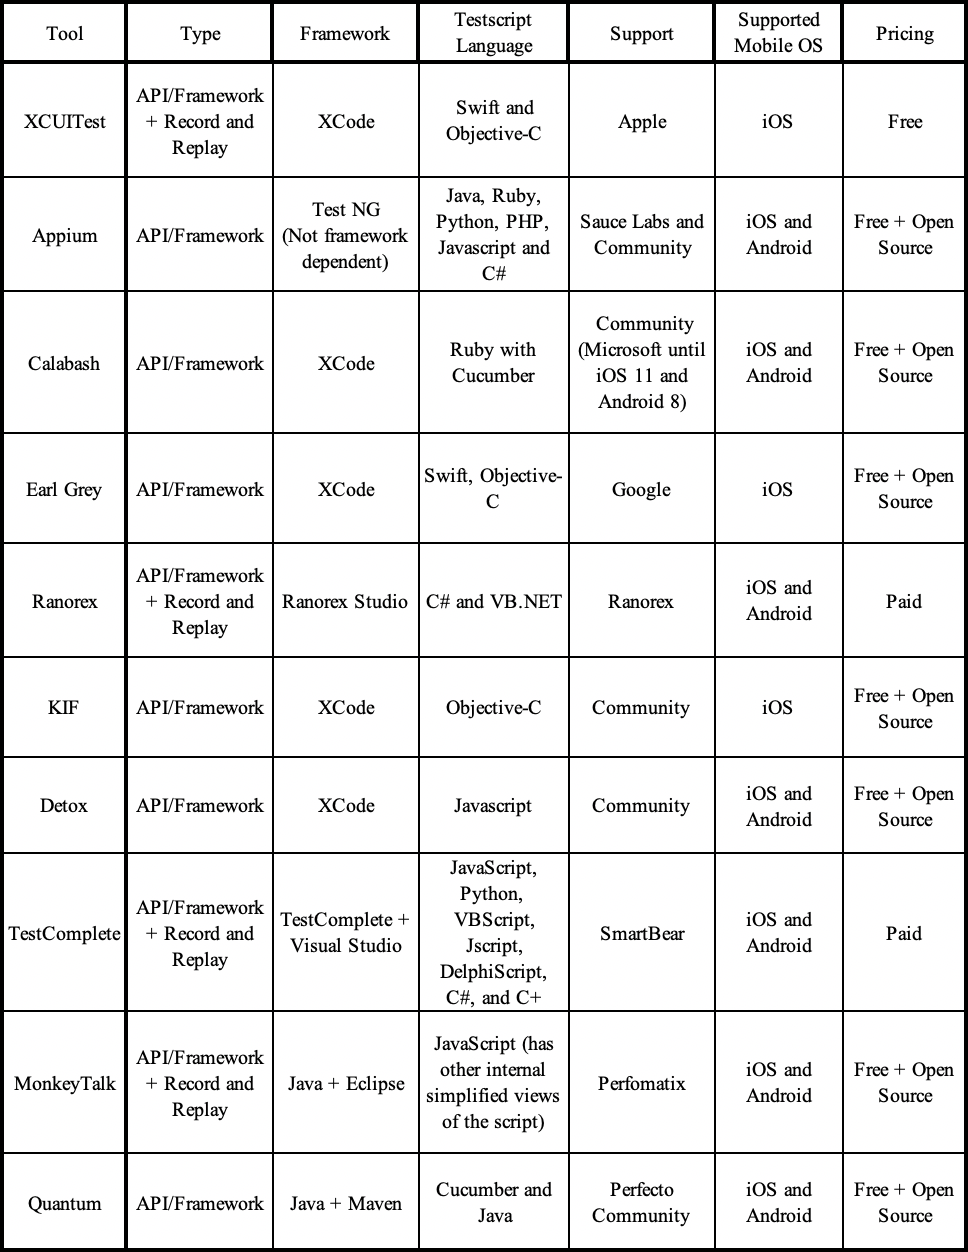
\includegraphics[width=12cm]{img/table1.png} \\[0mm]
	\vspace{0cm}
	\caption{General tool comparison table}
	\label{Toolcomparison}
\end{figure} 

\section{Categories}
In order to compare test automation tools, it is important to understand the different elements, interactions and functionality an iOS mobile app utilizes. These will be broken down in three categories: GUI components, Gestures and Testing Capabilities. The first makes reference to the all the elements that make up the graphical user interface, these are also divided into three categories: Bars, Views and Controls. Gestures are the way users interact with the touchscreen, this is the main way users provide input to their mobile devices. Finally, testing capabilities make reference to the various APIs the test automation tool could provide in order to manipulate the application OS and hardware configurations.

The following is a list of GUI components and gestures Apple has publicly defined [To-Link], as well as some of the testing capabilities that one may need while automating tests. 

\subsection {GUI Components}
	
	Bars
	\begin{itemize}
  		\vspace{-0.4cm}\item Navigation Bar
  		\vspace{-0.4cm}\item Search Bars
		\vspace{-0.4cm}\item Status Bars
		\vspace{-0.4cm}\item Tab Bars
		\vspace{-0.4cm}\item Toolbars
	\end{itemize}

	Views
	\begin{itemize}
  		\vspace{-0.4cm}\item Action Sheets
		\vspace{-0.4cm}\item Activity Views
		\vspace{-0.4cm}\item Alerts
		\vspace{-0.4cm}\item Collections
		\vspace{-0.4cm}\item Image Views
		\vspace{-0.4cm}\item Pages
		\vspace{-0.4cm}\item Popovers
		\vspace{-0.4cm}\item Scroll Views
		\vspace{-0.4cm}\item Split Views
		\vspace{-0.4cm}\item Tables
		\vspace{-0.4cm}\item Text Views
		\vspace{-0.4cm}\item Web Views
	\end{itemize}
	
	Controls
	\begin{itemize}
  		\vspace{-0.4cm}\item Buttons
		\vspace{-0.4cm}\item Context Menus
		\vspace{-0.4cm}\item Edit Menus
		\vspace{-0.4cm}\item Labels
		\vspace{-0.4cm}\item Page Controls
		\vspace{-0.4cm}\item Pickers
		\vspace{-0.4cm}\item Progress Indicators
		\vspace{-0.4cm}\item Refresh Content Controls
		\vspace{-0.4cm}\item Segmented Controls
		\vspace{-0.4cm}\item Sliders
		\vspace{-0.4cm}\item Steppers
		\vspace{-0.4cm}\item Switches
		\vspace{-0.4cm}\item Text Fields
	\end{itemize}

\subsection {Gestures}

	\begin{itemize}
  		\vspace{-0.4cm}\item 3D Touch
		\vspace{-0.4cm}\item Tap
		\vspace{-0.4cm}\item Drag
		\vspace{-0.4cm}\item Flick
		\vspace{-0.4cm}\item Swipe
		\vspace{-0.4cm}\item Double tap
		\vspace{-0.4cm}\item Pinch
		\vspace{-0.4cm}\item Touch and Hold
		\vspace{-0.4cm}\item Shake
		\vspace{-0.4cm}\item Rotate
	\end{itemize}

\subsection {Framework Testing Capabilities}
	\begin{itemize}
  		\vspace{-0.4cm}\item Element handling: Element searching and Element attributes
		\vspace{-0.4cm}\item Authentication: Touch ID and Face ID
		\vspace{-0.4cm}\item Toggle hardware configurations: Wi-Fi, Data, Bluetooth, …
		\vspace{-0.4cm}\item Access system configurations: Language, Region, Time, Text Size, …
		\vspace{-0.4cm}\item Change device orientation
		\vspace{-0.4cm}\item GPS mocking
		\vspace{-0.4cm}\item Camera mocking
		\vspace{-0.4cm}\item Application state (set app to background, reopen app)
		\vspace{-0.4cm}\item Multitasking
		\vspace{-0.4cm}\item Notification handling
		\vspace{-0.4cm}\item Access app cache  data
		\vspace{-0.4cm}\item File handling
	\end{itemize}
	
\subsection {Automation Tool Characteristics and Features}

Another important aspect to take into account when evaluating the suitability of a framework for a project is the characteristics and features the tool provides. There are certain characteristics or features besides the automated testing itself that may become invaluable. 

Examples for such are: 
	\begin{itemize}
  		\vspace{-0.4cm}\item Performance: Test execution time, memory use, …
		\vspace{-0.4cm}\item Maintainability
		\vspace{-0.4cm}\item Test parallelization
		\vspace{-0.4cm}\item Emulated and Real Device compatibility
		\vspace{-0.4cm}\item Ease of development (skill required)
		\vspace{-0.4cm}\item Android (hybrid) project compatibility
		\vspace{-0.4cm}\item Programming Languages Supported
		\vspace{-0.4cm}\item Developer Support
		\vspace{-0.4cm}\item Price
	\end{itemize}

 % INCLUDE: related work
\chapter{Case Study}
\label{chapter3}

For this project, a case study focused on taking a closer look into the popular XCUITest test automation framework and other XCTest based user interface test automation frameworks will be performed. In order to achieve this, an iOS application, a set of test cases and automated tests are needed.




\section{Wikipedia iOS App}
After exploring several open source applications, the Firefox project for iOS seemed to be the best fit, since it provides a big enough and stable application as well as hundreds of working automated UI tests. These automated tests make use of the XCUITest framework for black box testing along with KIF and EarlGrey for grey box testing. On the other hand, the project is currently up to date regarding the software versions used and it is constantly been worked on, which greatly reduces compatibility issues.

https://github.com/mozilla-mobile/firefox-ios

\section{Test Cases}
Considering the objective of this case study is to compare the different test automation tools, the following set of test cases aims to cover as many different situations one could encounter while testing, and not providing a coverage for the application itself. This means, they will try to cover as many of the GUI components, gestures and testing capabilities as possible within the existing automated tests in the Firefox App.

Test Cases: (In MS Excel document)

\section{Results}
The following tables provide, for each tool, a view which matches a specific GUI component, gesture or testing capability with a test case that involves it. This is particularly useful if you desire to explore a real-world example of an automated UI test for some of the different GUI components, gestures and framework testing capabilities or if you want to verify its coverage.


	\subsection{XCTestUI}
	(In MS Word document)
	
	
	\subsection{KIF}
	(In MS Word document)
	
	
	\subsection{EarlGrey}
	(In MS Word document)

After some extra research, the coverage of several GUI components, gestures and framework testing capabilities could be exhibited. However, these do not have a related test case as there is no automated test in the Firefox App to associate them with. It is also important to take into account the fact that not all GUI components, gestures and framework testing capabilities were evaluated.



	
	% INCLUDE: system
% !TEX root = ../thesis-example.tex
%
\chapter{Conclusion}
\label{chapter5}

During the development of this project t

\section{Objetives met}
Given the initial project objectives: Tool Research, Case Study, Documentation

\section{Limitations}
	\begin{itemize}
		\item Limited options for iOS open source apps.
		\item Time scope of the project was not enough to actually develop the case study with different types of automation tools.
		\item All in one tools can be very expensive. For example, TestComplete will easily cost more than 6,000 USD a year per user with no add-ons.
	\end{itemize}


\section{Future work}

This project has several opportunities for improvement:

	\begin{itemize}
		\item Performing the same Case Study content with more test automation tools. 
		\item Making use of more iOS applications in order to reference more real world test cases and automated test scripts.
		\item Expanding the coverage table, including more GUI components, gestures and testing capabilities for the used tools.
	\end{itemize}

 % INCLUDE: conclusion
\cleardoublepage

\printbibliography

\cleardoublepage
\clearpage

%\listoftables
%\clearpage

% !TEX root = ../thesis-example.tex
%
\pagestyle{empty}
\hfill
\vfill
\pdfbookmark[0]{Colophon}{Colophon}
\section*{Colophon}

This document was written in \LaTeXe. It utilizes the stile \textit{Clean Thesis} developed by Ricardo Langner.
%\cleardoublepage
%% !TEX root = ../thesis-example.tex
%
%************************************************
% Declaration
%************************************************
\pdfbookmark[0]{Declaration}{Declaration}
\chapter*{Declaration}
\label{sec:declaration}
\thispagestyle{empty}

You can put your declaration here, to declare that you have completed your work solely and only with the help of the references you mentioned.

\bigskip

\noindent\textit{\thesisUniversityCity, \thesisDate}

\smallskip

\begin{flushright}
	\begin{minipage}{5cm}
		\rule{\textwidth}{1pt}
		\centering\thesisName
	\end{minipage}
\end{flushright}

%*****************************************
%*****************************************

\clearpage
\newpage
\mbox{}

% **************************************************
% End of Document CONTENT
% **************************************************
\end{document}
